% Gabarit pandoc des corrigés publiés (brut et guidé). Contenu sans marque ni nom de site.
% Compilation : lualatex (latexmk -lualatex).
% Le Markdown reste la source unique : ne pas éditer ce fichier .tex à la main.
\documentclass[11pt,a4paper]{article}

% --- Moteur, polices (Latin Modern) et langue ---------------------------------
\usepackage{iftex}
\ifLuaTeX\else\errmessage{Ce document se compile avec lualatex}\fi
\usepackage{amsmath,amssymb,mathtools}
\usepackage{fontspec}
% mathrm=sym : \mathrm prend ses glyphes dans la police mathématique (ℓ, μ, Ω), comme KaTeX.
\usepackage[math-style=TeX,bold-style=TeX,mathrm=sym]{unicode-math}
% Repli pour les glyphes absents de Latin Modern (indices et exposants Unicode,
% flèches, filets des schémas en texte, symboles) : DejaVu, puis Latin Modern Math
% (ℓ, lettres mathématiques Unicode des légendes).
\directlua{
  luaotfload.add_fallback("repliTexte", {"DejaVuSerif:mode=harf;", "DejaVuSans:mode=harf;", "file:latinmodern-math.otf:mode=harf;"})
  luaotfload.add_fallback("repliMono", {"DejaVuSansMono:mode=harf;", "DejaVuSans:mode=harf;", "file:latinmodern-math.otf:mode=harf;"})
}
\setmainfont{Latin Modern Roman}[RawFeature={fallback=repliTexte}]
\setsansfont{Latin Modern Sans}[RawFeature={fallback=repliTexte}]
\setmonofont{Latin Modern Mono}[RawFeature={fallback=repliMono}]
\setmathfont{Latin Modern Math}
\usepackage[french]{babel}
\frenchsetup{SmallCapsFigTabCaptions=false}

% --- Mise en page --------------------------------------------------------------
\usepackage[a4paper,margin=2.2cm,headheight=14pt,footskip=1.2cm]{geometry}
\usepackage{microtype}
\setlength{\emergencystretch}{4em}
\tolerance=1500
\setlength{\parindent}{0pt}
\setlength{\parskip}{0.55\baselineskip plus 2pt minus 1pt}
\usepackage{xcolor}
% Gris nommés : babel-french rend « ! » actif dans le document.
\definecolor{gris2}{gray}{0.98}
\definecolor{gris3}{gray}{0.97}
\definecolor{gris5}{gray}{0.95}
\definecolor{gris35}{gray}{0.65}
\definecolor{gris40}{gray}{0.60}
\definecolor{gris45}{gray}{0.55}
\definecolor{gris50}{gray}{0.50}
\definecolor{gris55}{gray}{0.45}
\definecolor{gris60}{gray}{0.40}
\definecolor{gris65}{gray}{0.35}
\definecolor{gris70}{gray}{0.30}
\definecolor{gris80}{gray}{0.20}
\definecolor{gris85}{gray}{0.15}
\usepackage{graphicx}
\usepackage{float}
\usepackage{caption}
\captionsetup{font=small,labelformat=empty,justification=centering}
\usepackage{booktabs,longtable,array,multirow,calc}
\usepackage{siunitx}
\sisetup{locale=FR}
\usepackage[version=4]{mhchem}
\usepackage{listings}
\usepackage{fancyhdr}
\usepackage{lastpage}
\usepackage[most]{tcolorbox}
\usepackage{enumitem}
\setlist{nosep,leftmargin=*,topsep=2pt}
\usepackage[hidelinks,unicode]{hyperref}
\usepackage{bookmark}
\hypersetup{pdftitle={Banque PT 2026 — Physique B (thermodynamique)},pdfauthor={Rédigé par IA},pdfcreator={LaTeX},pdfsubject={Corrigé brut}}
\usepackage{xurl}

% --- Pandoc : listes, tableaux, figures ----------------------------------------
\providecommand{\passthrough}[1]{#1}
\providecommand{\tightlist}{\setlength{\itemsep}{0pt}\setlength{\parskip}{0pt}}

\makeatletter
\def\maxwidth{\ifdim\Gin@nat@width>\linewidth\linewidth\else\Gin@nat@width\fi}
\def\maxheight{\ifdim\Gin@nat@height>0.55\textheight 0.55\textheight\else\Gin@nat@height\fi}
\makeatother
\setkeys{Gin}{width=\maxwidth,height=\maxheight,keepaspectratio}
\setcounter{secnumdepth}{-\maxdimen}
\providecommand{\pandocbounded}[1]{#1}
\usepackage{longtable,booktabs,array}

% --- Code (listings) -----------------------------------------------------------
\lstset{
  basicstyle=\ttfamily\small,
  columns=fullflexible,
  keepspaces=true,
  breaklines=true,
  breakatwhitespace=false,
  postbreak=\mbox{\textcolor{gris50}{$\hookrightarrow$}\space},
  frame=single,
  rulecolor=\color{gris35},
  framesep=4pt,
  xleftmargin=5pt,xrightmargin=5pt,
  backgroundcolor=\color{gris3},
  keywordstyle=\bfseries,
  commentstyle=\color{gris65},
  stringstyle=\color{gris80},
  showstringspaces=false,
  tabsize=4,
  extendedchars=true,
  aboveskip=6pt,belowskip=6pt,
}

% --- Macros des corrigés (KaTeX ↔ LaTeX) ---------------------------------------
% Les corrigés sont écrits pour KaTeX : on définit ici ce que KaTeX connaît et
% que LaTeX n'a pas, sans jamais retoucher le Markdown.
\providecommand{\R}{\mathbb{R}}
\providecommand{\N}{\mathbb{N}}
\providecommand{\Z}{\mathbb{Z}}
\providecommand{\Q}{\mathbb{Q}}
\providecommand{\C}{\mathbb{C}}
\providecommand{\dd}{\mathrm{d}}
\providecommand{\llbracket}{\lBrack}
\providecommand{\rrbracket}{\rBrack}
\providecommand{\lBrace}{\lbrace}
\providecommand{\rBrace}{\rbrace}
\providecommand{\Box}{\square}
\providecommand{\Diamond}{\lozenge}
\providecommand{\varnothing}{\emptyset}
\providecommand{\argmax}{\operatorname*{arg\,max}}
\providecommand{\argmin}{\operatorname*{arg\,min}}
\renewcommand{\leq}{\leqslant}
\renewcommand{\geq}{\geqslant}

% Équation hors texte : réduite à la largeur de la ligne si elle déborde.
\newsavebox{\boiteequation}
\newcommand{\equationajustee}[1]{%
  \sbox{\boiteequation}{$\displaystyle #1$}%
  \ifdim\wd\boiteequation>\linewidth
    \[\resizebox{\linewidth}{!}{\usebox{\boiteequation}}\]%
  \else
    \[#1\]%
  \fi}

% --- Encadrés pédagogiques (sobres, lisibles en noir et blanc) -----------------
\tcbset{
  encadre/.style={
    enhanced,breakable,sharp corners,
    colback=white,colframe=gris55,
    boxrule=0.4pt,leftrule=2.2pt,
    left=6pt,right=6pt,top=3pt,bottom=3pt,
    before skip=6pt,after skip=6pt,
    fonttitle=\bfseries\small,coltitle=black,
    attach title to upper,after title={\quad},
    parbox=false,
  }
}
\newtcolorbox{indication}[1]{encadre,colframe=gris45,colback=gris2,title={Indication~#1}}
\newtcolorbox{methode}{encadre,colframe=gris70,title={Méthode}}
\newtcolorbox{piege}{encadre,colframe=gris85,boxrule=0.8pt,leftrule=2.2pt,title={Piège}}
\newtcolorbox{jury}{encadre,colframe=gris60,colback=gris5,title={Jury}}
\newtcolorbox{encadrenote}{encadre,colframe=gris40}

% --- Titres de section ---------------------------------------------------------
\usepackage{titlesec}
\titleformat{\section}{\Large\bfseries}{}{0pt}{}
\titleformat{\subsection}{\large\bfseries}{}{0pt}{}
\titleformat{\subsubsection}{\normalsize\bfseries}{}{0pt}{}
\titlespacing*{\section}{0pt}{14pt plus 4pt minus 2pt}{6pt}
\titlespacing*{\subsection}{0pt}{10pt plus 3pt minus 2pt}{4pt}
\titlespacing*{\subsubsection}{0pt}{8pt plus 2pt minus 2pt}{2pt}

% --- En-tête et pied de page ---------------------------------------------------
\pagestyle{fancy}
\fancyhf{}
\fancyhead[L]{\small\textsc{Corrigé brut} · Banque PT PT}
\fancyhead[R]{\small Physique B - thermodynamique 2026}
\fancyfoot[L]{\footnotesize Corrigé rédigé par IA, non officiel}
\fancyfoot[R]{\footnotesize \thepage\,/\,\pageref*{LastPage}}
\renewcommand{\headrulewidth}{0.4pt}
\renewcommand{\footrulewidth}{0pt}
\fancypagestyle{plain}{\fancyhf{}\fancyfoot[R]{\footnotesize \thepage\,/\,\pageref*{LastPage}}\fancyfoot[L]{\footnotesize Corrigé rédigé par IA, non officiel}\renewcommand{\headrulewidth}{0pt}}

\begin{document}
\thispagestyle{plain}
\begin{center}
  {\small\scshape Corrigé brut}\par\smallskip
  {\LARGE\bfseries Banque PT 2026 — Physique B (thermodynamique)\par}\medskip
  {\large Banque PT · PT · Physique B - thermodynamique · 2026\par}
\end{center}
\vspace{2pt}\hrule\vspace{8pt}

\emph{Corrigé rédigé par IA, non officiel. Signalez toute erreur.}

Épreuve de 2 h, calculatrice interdite, document réponse 1 (diagramme \((T,s)\) de l'eau et tableau) à rendre. Thème : le procédé MESMA de propulsion anaérobie des sous-marins.

\hypertarget{partie-1-description-thermodynamique-du-cycle}{%
\section{Partie 1 : Description thermodynamique du cycle}\label{partie-1-description-thermodynamique-du-cycle}}

\hypertarget{q1}{%
\subsection{Q1}\label{q1}}

\textbf{Système} : l'eau (fluide caloporteur) du circuit secondaire. On suit une masse donnée sur un cycle complet, ce qui en fait un système fermé qui revient à son état initial.

\textbf{Convention} : les échanges sont comptés algébriquement, positivement quand ils sont reçus par l'eau. Le signe obtenu indique ensuite le \textbf{sens réel} du transfert : positif si l'eau reçoit effectivement l'énergie, négatif si elle la cède.

\begin{itemize}
\tightlist
\item
  \(Q_c\) est reçu dans le \textbf{générateur de vapeur}, l'échangeur où les gaz de combustion éthanol/oxygène (source chaude, à \(T_{ch}\)) chauffent l'eau : \(Q_c>0\) ;
\item
  \(Q_f\) est reçu dans le \textbf{condenseur}, au contact de la source froide (eau de mer) à \(T_{fr}\) : \(Q_f<0\), car l'eau cède de la chaleur ;
\item
  \(W\) est le travail reçu, échangé avec l'arbre de la turbine (et de la pompe) : \(W<0\), car le dispositif est moteur.
\end{itemize}

\begin{figure}[H]
\centering
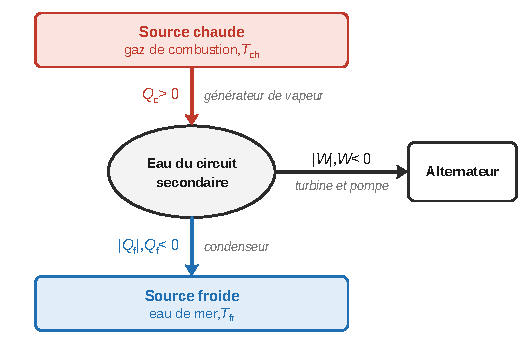
\includegraphics{figures/q01-echanges-moteur-ditherme.pdf}
\caption*{Figure 1 --- Échanges d'énergie de l'eau du circuit secondaire,
modélisée en moteur ditherme}
\end{figure}

Sur le schéma, les flèches donnent le sens réel des transferts : \(Q_c\) entre dans l'eau, \(|Q_f|\) et \(|W|\) en sortent. Le bilan s'écrit \(|W|=Q_c-|Q_f|\).

\hypertarget{q2}{%
\subsection{Q2}\label{q2}}

Le premier principe sur un cycle (\(\Delta U=0\)) donne \(W+Q_c+Q_f=0\).

Le second principe sur un cycle (\(\Delta S=0\)), pour un fonctionnement réversible (\(S_{\text{\text{créée}}}=0\)) avec deux thermostats, donne \(\dfrac{Q_c}{T_{ch}}+\dfrac{Q_f}{T_{fr}}=0\), soit \(Q_f=-Q_c\,\dfrac{T_{fr}}{T_{ch}}\).

Le rendement est le rapport entre l'énergie utile, le travail fourni \(-W>0\), et l'énergie coûteuse, le transfert \(Q_c\) reçu de la source chaude :
\equationajustee{\begin{aligned}
\eta&=\frac{-W}{Q_c}\\
&=\frac{Q_c+Q_f}{Q_c}\\
&=1+\frac{Q_f}{Q_c}
\end{aligned}}

Avec la relation tirée du second principe :
\equationajustee{\boxed{\eta_C=1-\frac{T_{fr}}{T_{ch}}}}

\hypertarget{q3}{%
\subsection{Q3}\label{q3}}

On convertit en kelvins : \(T_{ch}=773\) K et \(T_{fr}=373\) K.
\equationajustee{\begin{aligned}
\eta_C&=1-\frac{373}{773}\\
&\approx1-0{,}48
\end{aligned}}

\equationajustee{\boxed{\eta_C\approx0{,}52}}

\hypertarget{q4}{%
\subsection{Q4}\label{q4}}

Pour un cycle irréversible, le second principe s'écrit \(0=\dfrac{Q_c}{T_{ch}}+\dfrac{Q_f}{T_{fr}}+S_{\text{\text{créée}}}\), d'où \(Q_f=-T_{fr}\left(\dfrac{Q_c}{T_{ch}}+S_{\text{\text{créée}}}\right)\). On en déduit :
\equationajustee{\begin{aligned}
\eta&=1+\frac{Q_f}{Q_c}\\
&=1-\frac{T_{fr}}{T_{ch}}-\frac{T_{fr}\,S_{\text{\text{créée}}}}{Q_c}
\end{aligned}}

\equationajustee{\boxed{\eta=1-\frac{T_{fr}}{T_{ch}}-\frac{T_{fr}\,S_{\text{\text{créée}}}}{Q_c}}}

Le terme irréversible est homogène : \(T_{fr}\,S_{\text{\text{créée}}}\) est une énergie, comme \(Q_c\).

Comme \(S_{\text{\text{créée}}}\ge0\), on a \(\eta\le\eta_C\), avec égalité seulement pour un cycle réversible.

\hypertarget{q5}{%
\subsection{Q5}\label{q5}}

\textbf{Système} : on se donne un volume de contrôle fixe, par exemple un composant entre sa section d'entrée \(E\) et sa section de sortie \(S\). On définit le système fermé \(\Sigma\) :
- à l'instant \(t\), c'est le fluide contenu dans ce volume, augmenté de la masse \(\delta m\) qui va entrer pendant \(\mathrm{d}t\) ;
- à l'instant \(t+\mathrm{d}t\), c'est le fluide contenu dans ce volume, augmenté de la masse \(\delta m\) sortie.

La masse sortie est égale à la masse entrée, puisque le régime est stationnaire.

On applique le premier principe à \(\Sigma\). Le travail des forces de pression en amont et en aval vaut \((P_ev_e-P_sv_s)\,\delta m\). On obtient, par unité de masse :
\equationajustee{\boxed{\Delta h+\Delta\!\left(\frac{c^2}{2}\right)+g\,\Delta z=w_u+q}}

Les termes sont les suivants :
- \(h=u+Pv\) est l'enthalpie massique ;
- \(c\) est la vitesse d'ensemble du fluide et \(z\) son altitude ;
- \(w_u\) est le travail massique \textbf{utile}, échangé avec les parties mobiles (arbre de pompe ou de turbine), hors forces de pression d'entrée et de sortie ;
- \(q\) est le transfert thermique massique reçu.

Si l'on néglige l'énergie cinétique et la pesanteur :
\equationajustee{\boxed{h_s-h_e=w_u+q}}

Cela donne, pour chaque élément du circuit :
- dans la pompe et la turbine, adiabatiques : \(\Delta h=w_u\) ;
- dans le générateur et le condenseur, sans pièce mobile : \(\Delta h=q\).

\hypertarget{q6}{%
\subsection{Q6}\label{q6}}

On modélise l'eau liquide par une phase condensée incompressible et indilatable. Son entropie massique vaut alors \(s=c\ln T+\text{cste}\) et ne dépend que de \(T\). La compression 1→2 est isentropique, donc \(s_2=s_1\), d'où :
\equationajustee{\boxed{T_2=T_1=100\ ^\circ\text{C}}}

L'enthalpie varie peu : \(h_2-h_1=v\,(P_2-P_1)\approx10^{-3}\times49\times10^5\approx5\) kJ·kg⁻¹, donc \(h_2\approx445\) kJ·kg⁻¹.

\hypertarget{q7}{%
\subsection{Q7}\label{q7}}

\begin{itemize}
\tightlist
\item
  Le générateur de vapeur est isobare, donc \(\boxed{P_3=P_2=50\text{ bar}}\).
\item
  Le condenseur est isobare, donc \(\boxed{P_4=P_1=1\text{ bar}}\).
\item
  L'état 4 est un mélange liquide-vapeur en équilibre sous 1 bar, à la même pression que l'état 1, qui est un liquide saturé à 100 °C. Or la température d'équilibre ne dépend que de la pression, donc \(\boxed{T_4=T_1=100\ ^\circ\text{C}}\). La température de vaporisation de l'eau sous 1 bar vaut bien environ 100 °C.
\end{itemize}

\textbf{Allure du cycle dans le diagramme \((P,v)\)}, avec \(P\) en ordonnée, \(v\) en abscisse et la courbe de saturation en cloche :
- le point 1 est sur la branche liquide de la cloche, à \(P=1\) bar ;
- 1→2 est un segment quasi vertical (le liquide est quasi incompressible) qui monte jusqu'à 50 bar, à gauche de la cloche ;
- 2→3 est l'isobare horizontale à 50 bar. Elle comporte l'échauffement du liquide jusqu'à la courbe d'ébullition, puis le palier de vaporisation sous la cloche (à environ 264 °C), puis la surchauffe de la vapeur jusqu'à 500 °C, à droite de la cloche ;
- 3→4 est la détente isentropique, une courbe décroissante plus raide qu'une isotherme. Elle entre dans la cloche et s'arrête au point 4, près de la branche vapeur ;
- 4→1 est le palier horizontal à 1 bar sous la cloche, de 4 jusqu'à 1.

Le cycle est parcouru dans le sens horaire, ce qui correspond à un cycle moteur.

\begin{figure}[H]
\centering
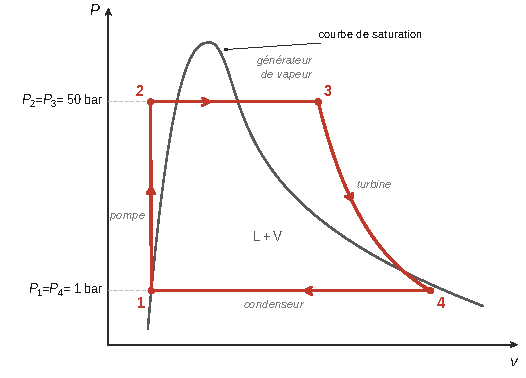
\includegraphics{figures/q07-cycle-clapeyron.pdf}
\caption*{Figure 2 --- Allure du cycle dans le diagramme de Clapeyron (P, v),
parcouru dans le sens horaire}
\end{figure}

\hypertarget{q8}{%
\subsection{Q8}\label{q8}}

Pour un gaz parfait, \(\mathrm{d}h=c_p\,\mathrm{d}T=T\,\mathrm{d}s+v\,\mathrm{d}P\). Sur une isobare, \(\mathrm{d}T/T=\mathrm{d}s/c_p\). Si \(c_p\) est constant :
\equationajustee{\boxed{T=T_0\exp\!\left(\frac{s-s_0}{c_p}\right)}}

Les isobares sont donc des exponentielles croissantes. Comme \((\partial s/\partial P)_T=-r/P<0\), les isobares de haute pression sont décalées vers la gauche.

Pour un gaz parfait, \(h\) ne dépend que de \(T\) (deuxième loi de Joule) : les isenthalpes sont des isothermes, donc des \textbf{droites horizontales} dans le diagramme \((T,s)\). À entropie élevée, c'est-à-dire à basse pression et loin de la courbe de saturation, la vapeur d'eau se comporte comme un gaz parfait. Les isenthalpes du diagramme y deviennent \textbf{horizontales}, comme on le voit en haut à droite du document réponse.

\hypertarget{q9}{%
\subsection{Q9}\label{q9}}

Placement des points sur le document réponse 1 :

\begin{longtable}[]{@{}
  >{\raggedright\arraybackslash}p{(\columnwidth - 2\tabcolsep) * \real{0.1175}}
  >{\raggedright\arraybackslash}p{(\columnwidth - 2\tabcolsep) * \real{0.8525}}@{}}
\toprule\noalign{}
\begin{minipage}[b]{\linewidth}\raggedright
Point
\end{minipage} & \begin{minipage}[b]{\linewidth}\raggedright
Position sur le diagramme \((T,s)\)
\end{minipage} \\
\midrule\noalign{}
\endhead
\bottomrule\noalign{}
\endlastfoot
1 & Sur la courbe d'ébullition (branche gauche), à \(T=100\) °C et \(s_1=1{,}3\) kJ·kg⁻¹·K⁻¹. \\
2 & À la verticale de 1 (\(s_2=s_1\)), à \(T_2=100\) °C, sur l'isobare 5 MPa. Dans le domaine liquide, les isobares se confondent pratiquement avec la courbe d'ébullition, donc 2 est quasiment confondu avec 1. \\
3 & Intersection de l'isobare 5 MPa et de l'isotherme 500 °C, nettement à droite de la cloche, vers \(s_3\approx7{,}0\) kJ·kg⁻¹·K⁻¹. L'isobare 5 MPa (50 bar) est la courbe repérée « 5 » sur l'échelle des pressions en haut du diagramme, entre les isobares 10 MPa et 2 MPa. \\
4 & À la verticale de 3 (\(s_4=s_3\), détente adiabatique réversible), sur l'isotherme 100 °C, dans la cloche, entre la courbe \(q=0{,}9\) et la courbe de rosée. \\
\end{longtable}

Le cycle se compose de quatre portions :
- 1→2 est réduit à un point ;
- 2→3 suit l'isobare 5 MPa : montée le long de la courbe d'ébullition jusqu'à environ 264 °C, palier horizontal de vaporisation dans la cloche jusqu'à la courbe de rosée, puis montée exponentielle dans la vapeur sèche jusqu'à 500 °C ;
- 3→4 est un segment vertical ;
- 4→1 est un segment horizontal à 100 °C.

\begin{figure}[H]
\centering
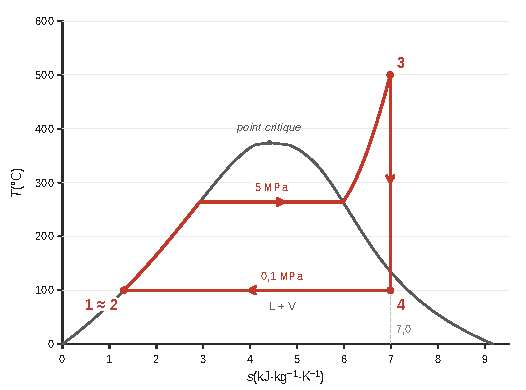
\includegraphics{figures/q09-cycle-diagramme-ts.pdf}
\caption*{Figure 3 --- Cycle dans le diagramme (T, s) de l'eau : 1 et 2 confondus,
palier à 5 MPa, détente verticale à s ≈ 7,0}
\end{figure}

\hypertarget{q10}{%
\subsection{Q10}\label{q10}}

L'état 2 est un \textbf{liquide comprimé} (sous-refroidi) : à 50 bar, la température de saturation (environ 264 °C) dépasse largement \(T_2=100\) °C. L'état 3 est une \textbf{vapeur sèche surchauffée}, puisque \(500\) °C est supérieur à la température de saturation à 50 bar.

Tableau complété par lecture graphique :

\begin{longtable}[]{@{}
  >{\raggedright\arraybackslash}p{(\columnwidth - 8\tabcolsep) * \real{0.1772}}
  >{\raggedright\arraybackslash}p{(\columnwidth - 8\tabcolsep) * \real{0.1712}}
  >{\raggedright\arraybackslash}p{(\columnwidth - 8\tabcolsep) * \real{0.1830}}
  >{\raggedright\arraybackslash}p{(\columnwidth - 8\tabcolsep) * \real{0.2241}}
  >{\raggedright\arraybackslash}p{(\columnwidth - 8\tabcolsep) * \real{0.2146}}@{}}
\toprule\noalign{}
\begin{minipage}[b]{\linewidth}\raggedright
\end{minipage} & \begin{minipage}[b]{\linewidth}\raggedright
1
\end{minipage} & \begin{minipage}[b]{\linewidth}\raggedright
2
\end{minipage} & \begin{minipage}[b]{\linewidth}\raggedright
3
\end{minipage} & \begin{minipage}[b]{\linewidth}\raggedright
4
\end{minipage} \\
\midrule\noalign{}
\endhead
\bottomrule\noalign{}
\endlastfoot
\(h\) (kJ·kg⁻¹) & 440 & \(\approx445\) & \(\approx3430\) & 2550 \\
\(s\) (kJ·kg⁻¹·K⁻¹) & 1,3 & 1,3 & \(\approx7{,}0\) & \(\approx7{,}0\) \\
état & liquide saturé & liquide comprimé & vapeur sèche surchauffée & mélange liquide-vapeur \\
\end{longtable}

\hypertarget{q11}{%
\subsection{Q11}\label{q11}}

L'entropie est une grandeur extensive. Pour un mélange de titre massique en vapeur \(x\) à la température \(T\) :
\equationajustee{\boxed{s(T)=x\,s_V(T)+(1-x)\,s_l(T)}}

On en déduit le titre :
\equationajustee{x=\frac{s-s_l}{s_V-s_l}}

La détente est adiabatique et réversible, donc \(s_4=s_3\approx7{,}0\) kJ·kg⁻¹·K⁻¹. Avec les données à \(T_4=T_1\) :
\equationajustee{\begin{aligned}
x_4&=\frac{s_4-s_l(T_1)}{s_V(T_1)-s_l(T_1)}\\
&=\frac{7{,}0-1{,}3}{7{,}3-1{,}3}\\
&=\frac{5{,}7}{6{,}0}
\end{aligned}}

\equationajustee{\boxed{x_4\approx0{,}95}}

L'aide numérique de l'énoncé, \(5{,}8/6{,}3\approx0{,}92\), ne correspond pas aux valeurs \(s_l=1{,}3\) et \(s_V=7{,}3\) fournies, dont la différence vaut 6,0. Elle conduirait à \(x_4\approx0{,}92\). Les deux valeurs restent dans l'incertitude de lecture.

\textbf{Lecture directe} : le point 4 se trouve sur l'isotherme 100 °C, entre la courbe \(q=0{,}9\) et la courbe de vapeur saturée, un peu plus près de la courbe \(0{,}9\). On lit \(x_4\approx0{,}93\) à \(0{,}95\), ce qui concorde avec le calcul.

\hypertarget{q12}{%
\subsection{Q12}\label{q12}}

D'après le premier principe industriel, sans travail utile, on a \(q=\Delta h\).

Générateur de vapeur (2→3) :
\equationajustee{\begin{aligned}
q_{23}&=h_3-h_2\\
&\approx3430-445
\end{aligned}}

\equationajustee{\boxed{q_{23}\approx2{,}99\times10^3\ \text{kJ·kg}^{-1}>0}}

Condenseur (4→1) :
\equationajustee{\begin{aligned}
q_{41}&=h_1-h_4\\
&=440-2550
\end{aligned}}

\equationajustee{\boxed{q_{41}\approx-2{,}11\times10^3\ \text{kJ·kg}^{-1}<0}}

Les signes sont ceux annoncés en Q1, avec la même convention (transfert reçu par l'eau) : \(q_{23}\) correspond à \(Q_c>0\) et \(q_{41}\) à \(Q_f<0\). Le fluide reçoit effectivement de la chaleur de la source chaude et en cède réellement à la source froide (l'eau de mer), ce qui est cohérent avec un moteur.

\hypertarget{q13}{%
\subsection{Q13}\label{q13}}

Sur un cycle, \(\Delta h=0\), donc \(w_{\text{cycle}}+q_{23}+q_{41}=0\) :
\equationajustee{\begin{aligned}
w_{\text{cycle}}&=-(q_{23}+q_{41})\\
&\approx-(2985-2110)
\end{aligned}}

\equationajustee{\boxed{w_{\text{cycle}}\approx-875\ \text{kJ·kg}^{-1}}}

Dans la turbine, adiabatique :
\equationajustee{\begin{aligned}
w_T&=h_4-h_3\\
&\approx2550-3430
\end{aligned}}

\equationajustee{\boxed{w_T\approx-880\ \text{kJ·kg}^{-1}}}

Les deux grandeurs portent sur le même cycle de Rankine : l'écart ne vient pas d'une irréversibilité. Le travail du cycle comprend aussi le travail reçu dans la pompe :
\equationajustee{w_P=h_2-h_1\approx+5\ \text{kJ·kg}^{-1}}

On a donc \(w_{\text{cycle}}=w_T+w_P\), et \(|w_{\text{cycle}}|<|w_T|\) : une partie du travail fourni par la turbine est consommée pour comprimer l'eau. Ce travail de pompe reste faible (moins de 1 \% de \(|w_T|\)), car on comprime un liquide de faible volume massique.

\hypertarget{q14}{%
\subsection{Q14}\label{q14}}

À la sortie de la turbine, le fluide est un \textbf{mélange liquide-vapeur} de titre \(x_4\approx0{,}95\), soit environ 5 \% de liquide en masse sous forme de gouttelettes. Ces gouttelettes, entraînées à grande vitesse, heurtent les aubes de la turbine. Elles provoquent une \textbf{érosion} et des chocs mécaniques sur les derniers étages, favorisent la corrosion et dégradent le rendement de la détente. C'est pourquoi on limite l'humidité en fin de détente (surchauffe, resurchauffe).

\hypertarget{q15}{%
\subsection{Q15}\label{q15}}

Le rendement est le travail utile fourni par le fluide divisé par la chaleur reçue de la source chaude :
\equationajustee{\eta=\frac{-w_{\text{cycle}}}{q_{23}}}

Application numérique :
\equationajustee{\eta\approx\frac{875}{2985}\approx0{,}29}

\equationajustee{\boxed{\eta\approx0{,}3}}

On a \(\eta\approx0{,}3<\eta_C\approx0{,}52\), ce qui est conforme à Q4 : le cycle réel crée de l'entropie. L'irréversibilité principale se situe dans le générateur de vapeur. L'eau y reçoit de la chaleur alors que sa température varie de 100 °C à 500 °C, au contact d'une source à \(T_{ch}\) : l'écart de température est fini. Au condenseur, au contraire, l'échange se fait à 100 °C, la température de la source froide.

\hypertarget{q16}{%
\subsection{Q16}\label{q16}}

On remonte la chaîne de conversion :
- puissance électrique : \(P_e=P_{\text{\text{méca}}}/0{,}8=250\) kW ;
- puissance mécanique fournie par la turbine à l'alternateur : \(P_T=P_e/0{,}95\approx263\) kW ;
- débit massique d'eau : \(P_T=D_m\,|w_T|\).

\equationajustee{D_m=\frac{P_{\text{\text{méca}}}}{0{,}8\times0{,}95\times|w_T|}}

Application numérique, avec les puissances en kW et le travail en kJ·kg⁻¹ :
\equationajustee{D_m\approx\frac{263}{880}}

\equationajustee{\boxed{D_m\approx0{,}3\ \text{kg·s}^{-1}}}

Le résultat est le même avec le travail net du cycle (875 kJ·kg⁻¹).

\hypertarget{partie-2-utilisation-de-loxyguxe8ne-liquide}{%
\section{Partie 2 : Utilisation de l'oxygène liquide}\label{partie-2-utilisation-de-loxyguxe8ne-liquide}}

\hypertarget{q17}{%
\subsection{Q17}\label{q17}}

\textbf{Homogénéité.} Le logarithme est sans dimension. D'après la loi de Fourier, \(\vec{j}_Q=-\lambda\,\overrightarrow{\mathrm{grad}}\,T\), la conductivité \(\lambda_a\) s'exprime en W·m⁻¹·K⁻¹. Donc \(\lambda_aL\) s'exprime en W·K⁻¹ et \(R_{th1}\) en K·W⁻¹. C'est bien l'unité d'une résistance thermique, rapport d'un écart de température à un flux.

\textbf{Pertinence.}
- \(R_{th1}\propto1/\lambda_a\) : à écart de température donné, un matériau plus conducteur laisse passer un flux plus grand, donc isole moins bien.
- \(R_{th1}\propto1/L\) : une conduite plus longue offre une surface de contact plus grande, donc un flux plus grand. Des tronçons placés côte à côte se comportent comme des résistances en parallèle.
- \(R_{th1}\) croît avec \(r_2/r_1\), donc avec l'épaisseur de la paroi que la chaleur doit traverser.
- Pour une paroi mince d'épaisseur \(\varepsilon=r_2-r_1\ll r_1\), on a \(\ln(r_2/r_1)\approx\varepsilon/r_1\). On retrouve la résistance \(\varepsilon/(\lambda S)\) d'un mur plan de surface \(S=2\pi r_1L\) :
\equationajustee{R_{th1}\approx\frac{\varepsilon}{\lambda_a\,2\pi r_1L}}

\textbf{Isolant}, de rayon intérieur \(r_2\), de rayon extérieur \(r_2+e\) et de conductivité \(\lambda_i\) :
\equationajustee{\boxed{R_{th2}=\frac{\ln\!\left(\dfrac{r_2+e}{r_2}\right)}{2\pi\lambda_iL}}}

\hypertarget{q18}{%
\subsection{Q18}\label{q18}}

D'après la loi de Newton, \(P=h_{ext}S\,(T_{ext}-T_S)=\dfrac{T_{ext}-T_S}{R_{cc}}\), où \(S=2\pi(r_2+e)L\) est la surface extérieure de l'isolant :
\equationajustee{\boxed{R_{cc}=\frac{1}{2\pi h_{ext}(r_2+e)L}}}

Le même flux \(\Phi\) traverse successivement la conduite, l'isolant puis la couche d'air, en régime stationnaire et sans accumulation aux interfaces. Les trois résistances sont donc en série :
\equationajustee{\boxed{R_{th-eq}=\frac{\ln(r_2/r_1)}{2\pi\lambda_aL}+\frac{\ln\!\left(\frac{r_2+e}{r_2}\right)}{2\pi\lambda_iL}+\frac{1}{2\pi h_{ext}(r_2+e)L}}}

\begin{figure}[H]
\centering
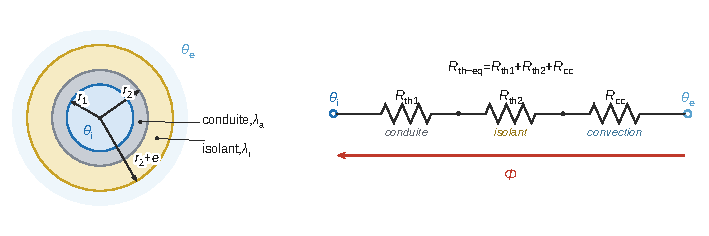
\includegraphics{figures/q18-resistances-serie.pdf}
\caption*{Figure 4 --- Conduite isolée en coupe et schéma équivalent : trois
résistances thermiques en série}
\end{figure}

\hypertarget{q19}{%
\subsection{Q19}\label{q19}}

Le flux est compté positivement de l'extérieur vers l'oxygène :
\equationajustee{\Phi=\frac{\theta_e-\theta_i}{R_{th-eq}}}

Avec l'expression de Q18 :
\equationajustee{\boxed{\Phi=\frac{2\pi L\,(\theta_e-\theta_i)}{\dfrac{\ln(r_2/r_1)}{\lambda_a}+\dfrac{\ln\left(1+e/r_2\right)}{\lambda_i}+\dfrac{1}{h_{ext}(r_2+e)}}}}

Avec la valeur fournie \(R_{th-eq}=1{,}0\) K·W⁻¹, on obtient \(\Phi=205/1{,}0\approx2\times10^2\) W, qui entrent dans l'oxygène.

\hypertarget{q20}{%
\subsection{Q20}\label{q20}}

Seuls les deux derniers termes de \(R_{th-eq}\) dépendent de \(e\). On pose \(r=r_2+e\) :
\equationajustee{\frac{\mathrm{d}R_{th-eq}}{\mathrm{d}e}=\frac{1}{2\pi L}\left(\frac{1}{\lambda_i r}-\frac{1}{h_{ext}r^2}\right)=\frac{1}{2\pi L\,\lambda_i r^2}\left(r-\frac{\lambda_i}{h_{ext}}\right)}

La dérivée s'annule pour le \textbf{rayon critique} \(r_c=\lambda_i/h_{ext}\), ce qui s'écrit aussi \(\alpha=\dfrac{h_{ext}r_2}{\lambda_i}=\dfrac{r_2}{r_c}\).

\begin{itemize}
\tightlist
\item
  \textbf{Cas \(\alpha>1\)}, soit \(r_2>r_c\) : pour tout \(e\ge0\), on a \(r>r_c\). La résistance \(R_{th-eq}\) est donc \textbf{strictement croissante} en \(e\) et augmente indéfiniment, de façon logarithmique.
\item
  \textbf{Cas \(\alpha<1\)}, soit \(r_2<r_c\) : la résistance \textbf{décroît} pour \(0\le e<e_c\), passe par un \textbf{minimum} en \(e_c\), puis croît. L'épaisseur critique vaut :
  \equationajustee{\begin{aligned}
  e_c&=r_c-r_2\\
  &=r_2\left(\frac1\alpha-1\right)
  \end{aligned}}
\end{itemize}

\begin{figure}[H]
\centering
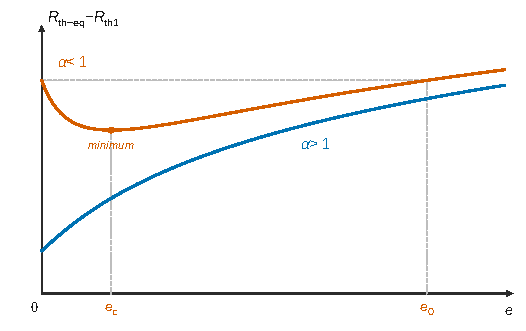
\includegraphics{figures/q20-rayon-critique.pdf}
\caption*{Figure 5 --- Allure de R\_th−eq(e) dans les cas α \textgreater{} 1 et α
\textless{} 1 (rayon critique)}
\end{figure}

\hypertarget{q21}{%
\subsection{Q21}\label{q21}}

Une fine couche supplémentaire d'isolant, d'épaisseur \(\mathrm{d}e\) posée sur le rayon \(r_2\), a deux effets opposés :
- elle ajoute une résistance de conduction \(\dfrac{\mathrm{d}e}{2\pi\lambda_i r_2L}\) ;
- elle agrandit la surface d'échange avec l'air, ce qui diminue la résistance de convection de \(\dfrac{\mathrm{d}e}{2\pi h_{ext}r_2^2L}\).

Le rapport du premier effet au second vaut \(\alpha=h_{ext}r_2/\lambda_i\). Le nombre \(\alpha\) indique donc quel phénomène limite le transfert thermique : la conduction dans l'isolant si \(\alpha>1\), la convection à la surface extérieure si \(\alpha<1\), c'est-à-dire si \(h_{ext}<\lambda_i/r_2\).

\begin{itemize}
\tightlist
\item
  \textbf{Si \(\alpha>1\)}, l'isolant est \textbf{toujours utile} : toute épaisseur augmente \(R_{th-eq}\) et diminue le flux entrant. C'est le cas usuel pour une conduite de quelques centimètres de rayon, puisque \(r_c=\lambda_i/h_{ext}\) vaut de l'ordre de quelques millimètres pour un bon isolant (\(\lambda_i\sim0{,}04\) W·m⁻¹·K⁻¹ et \(h_{ext}\sim10\) W·m⁻²·K⁻¹).
\item
  \textbf{Si \(\alpha<1\)}, la déperdition à la surface est limitante et une couche mince d'isolant est \textbf{néfaste}. L'augmentation de la surface d'échange convective l'emporte sur la résistance de conduction ajoutée, et le flux augmente. L'isolant ne devient utile qu'au-delà d'une épaisseur \(e_0>e_c\) telle que \(R_{th-eq}(e_0)=R_{th-eq}(0)\). Pour isoler, il faut alors choisir une épaisseur nettement supérieure à \(e_0\), ou un matériau de plus faible \(\lambda_i\), ce qui augmente \(\alpha\).
\end{itemize}

\hypertarget{q22}{%
\subsection{Q22}\label{q22}}

D'autres effets sont à surveiller :
- la \textbf{vaporisation} partielle de l'oxygène dans la conduite (point chaud, chute de pression, cavitation), qui donne un écoulement diphasé, perturbe le débit et la mesure, et peut créer des bouchons de vapeur ;
- le \textbf{givre} et la condensation de l'humidité de l'air sur les parois froides ;
- la \textbf{contraction thermique} de la conduite à −185 °C, qui crée des contraintes aux brides et aux supports ;
- la \textbf{fragilisation} des matériaux à basse température (transition ductile-fragile) ;
- le \textbf{risque d'incendie}. L'oxygène n'est pas lui-même inflammable : c'est un \textbf{comburant} puissant, qui entretient et accélère la combustion des matériaux \textbf{combustibles} à son contact (graisses, joints, isolants organiques). Il faut donc exclure les graisses, choisir des matériaux compatibles et surveiller les fuites ;
- les \textbf{pertes de charge} et l'étanchéité.

\hypertarget{q23}{%
\subsection{Q23}\label{q23}}

On suppose la vitesse uniforme sur chaque section. L'écoulement étant \textbf{stationnaire}, la masse contenue entre les sections A et B ne varie pas : le débit massique se conserve.
\equationajustee{\rho_A\,u\,S=\rho_B\,v\,s}

Le fluide étant de plus \textbf{incompressible}, \(\rho_A=\rho_B=\rho_d\), et c'est le débit volumique qui se conserve :
\equationajustee{uS=vs}

\equationajustee{\boxed{v=\frac{S}{s}\,u}}

On a \(v>u\) puisque \(s<S\).

\hypertarget{q24}{%
\subsection{Q24}\label{q24}}

Conditions d'application : écoulement \textbf{stationnaire} d'un fluide \textbf{parfait} (non visqueux), \textbf{incompressible} et homogène, sans pièce mobile ni échange thermique, entre deux points d'une même \textbf{ligne de courant}. Sous ces conditions :
\equationajustee{\boxed{P+\frac12\rho c^2+\rho g z=\text{cste le long d'une ligne de courant}}}

\hypertarget{q25}{%
\subsection{Q25}\label{q25}}

On applique Bernoulli entre A et B, sur une même ligne de courant et à la même altitude puisque le débitmètre est horizontal :
\equationajustee{P_A+\frac12\rho_du^2=P_B+\frac12\rho_dv^2}

Avec \(v=uS/s\) :
\equationajustee{\begin{aligned}
P_A-P_B&=\frac12\rho_d\left(v^2-u^2\right)\\
&=\frac12\rho_du^2\,\frac{S^2-s^2}{s^2}
\end{aligned}}

\equationajustee{\boxed{u=s\sqrt{\frac{2(P_A-P_B)}{\rho_d\,(S^2-s^2)}}}}

\hypertarget{q26}{%
\subsection{Q26}\label{q26}}

\equationajustee{\boxed{D_m=\rho_dSu=Ss\sqrt{\frac{2\rho_d(P_A-P_B)}{S^2-s^2}}}}

Application numérique, en unités SI :
- \(S=27\times10^{-4}\) m² et \(s=3\times10^{-4}\) m² ;
- \(P_A-P_B=0{,}044\) bar \(=4{,}4\times10^3\) Pa ;
- \(\rho_d=1100\) kg·m⁻³.

Comme \((s/S)^2=1/81\), on peut écrire \(S^2-s^2\approx S^2\). L'erreur vaut environ 1 \% sur \(S^2\) et 0,6 \% sur \(D_m\). On obtient alors \(D_m\approx s\sqrt{2\rho_d\Delta P}\), que l'on calcule à la main :
\equationajustee{\begin{aligned}
2\rho_d\Delta P&=2\times1100\times4400\\
&\approx9{,}7\times10^6\ \text{kg}^2\cdot\text{m}^{-4}\cdot\text{s}^{-2}\\
\sqrt{2\rho_d\Delta P}&\approx3{,}1\times10^3\ \text{kg}\cdot\text{m}^{-2}\cdot\text{s}^{-1}
\end{aligned}}

La dernière ligne utilise \(3{,}1^2=9{,}61\approx9{,}7\). D'où :
\equationajustee{\begin{aligned}
D_m&\approx3\times10^{-4}\times3{,}1\times10^3\\
&\approx0{,}93\ \text{kg·s}^{-1}
\end{aligned}}

Sans l'approximation \(S^2-s^2\approx S^2\), on trouverait \(0{,}94\) kg·s⁻¹.

\equationajustee{\boxed{D_m\approx1\ \text{kg·s}^{-1}}}

\hypertarget{q27}{%
\subsection{Q27}\label{q27}}

Pour un fluide réel, visqueux, deux types de pertes de charge apparaissent :
- des \textbf{pertes de charge régulières}, dues au frottement visqueux le long des parois (cylindre d'entrée, convergent, col, divergent) ;
- des \textbf{pertes de charge singulières}, dues aux changements de section, surtout dans le \textbf{divergent}, où l'écoulement peut se détacher des parois et former des tourbillons. Le convergent en provoque peu.

La pression en aval ne remonte donc pas à \(P_A\), et la relation de Q26 surestime légèrement le débit.

\hypertarget{uxe9volution-de-la-tempuxe9rature-le-long-de-la-conduite}{%
\section{Évolution de la température le long de la conduite}\label{uxe9volution-de-la-tempuxe9rature-le-long-de-la-conduite}}

\hypertarget{q28}{%
\subsection{Q28}\label{q28}}

\textbf{Système} : la tranche de fluide comprise entre \(x\) et \(x+\mathrm{d}x\), en régime permanent.

La résistance thermique est inversement proportionnelle à la longueur. Une tranche de longueur \(\mathrm{d}x\) a donc pour résistance \(R_{th-eq}L/\mathrm{d}x\), et elle reçoit de l'extérieur la puissance :
\equationajustee{\delta\Phi=\frac{\theta_e-\theta(x)}{R_{th-eq}\,L}\,\mathrm{d}x}

Le premier principe industriel s'applique sans travail utile, en négligeant l'énergie cinétique et la pesanteur. Pour un liquide, \(\mathrm{d}h=c_{dio}\,\mathrm{d}\theta\). On obtient \(D_m\,c_{dio}\,[\theta(x+\mathrm{d}x)-\theta(x)]=\delta\Phi\), soit :
\equationajustee{\boxed{\frac{\mathrm{d}\theta}{\mathrm{d}x}+\frac{\theta}{D_m\,c_{dio}\,R_{th-eq}\,L}=\frac{\theta_e}{D_m\,c_{dio}\,R_{th-eq}\,L}}}

\hypertarget{q29}{%
\subsection{Q29}\label{q29}}

L'équation s'écrit \(\dfrac{\mathrm{d}\theta}{\mathrm{d}x}+\dfrac{\theta}{\delta}=\dfrac{\theta_e}{\delta}\), avec :
\equationajustee{\boxed{\delta=D_m\,c_{dio}\,R_{th-eq}\,L}}

Vérification d'homogénéité : le produit \(D_m\,c_{dio}\,R_{th-eq}\) s'exprime en (kg·s⁻¹)(J·kg⁻¹·K⁻¹)(K·s·J⁻¹), donc il est sans dimension, et \(\delta\) est bien une longueur.

Application numérique : \(\delta=1\times1{,}7\times10^3\times1{,}0\times2\), donc
\equationajustee{\boxed{\delta\approx3{,}4\times10^3\ \text{m}\approx3\ \text{km}}}

\hypertarget{q30}{%
\subsection{Q30}\label{q30}}

Avec \(\theta(0)=\theta_i\), la solution est \(\theta(x)=\theta_e+(\theta_i-\theta_e)\,e^{-x/\delta}\). La variation sur la longueur \(L\) vaut donc :
\equationajustee{\boxed{\Delta\theta=\theta(L)-\theta_i=(\theta_e-\theta_i)\left(1-e^{-L/\delta}\right)}}

Elle est négligeable lorsque \(L\ll\delta\). On a alors, au premier ordre en \(L/\delta\) :
\equationajustee{\begin{aligned}
\Delta\theta&\approx(\theta_e-\theta_i)\,\frac{L}{\delta}\\
&=\frac{\theta_e-\theta_i}{D_m\,c_{dio}\,R_{th-eq}}
\end{aligned}}

Application numérique : \(L/\delta\approx6\times10^{-4}\), d'où
\equationajustee{\Delta\theta\approx\frac{205}{1700}}

\equationajustee{\boxed{\Delta\theta\approx0{,}12\ \text{K}}}

\textbf{Conclusion} : sur les quelques mètres de conduite d'un sous-marin, l'oxygène se réchauffe d'un dixième de kelvin environ. Il reste bien en dessous de sa température d'ébullition, qui est d'environ −183 °C sous 1 bar et plus élevée sous pression. Les conduites isolées du procédé MESMA (\(R_{th-eq}=1\) K·W⁻¹) remplissent leur rôle : l'oxygène arrive liquide au vaporisateur, à température quasi uniforme. Cela valide aussi l'hypothèse \(\theta_i\) uniforme des questions Q17 à Q21.

\end{document}
